\documentclass[aspectratio=169,10pt]{beamer}

\usetheme{dresden}
\usecolortheme{default}

\usepackage[utf8]{inputenc}
%\usepackage[T1]{fontenc}
\usepackage[ngerman]{babel}
\usepackage{amsmath}
\usepackage{booktabs}
\usepackage{tikz}
\usepackage{wrapfig}
\usepackage{graphics}

\graphicspath{images}

\usetikzlibrary{positioning,arrows.meta,spy,decorations.fractals,shadows,shapes.symbols}

\tikzset{
	rect/.style = {rectangle, minimum width = 5cm, minimum height = 0.75cm, thick},
}

\title{Abschlusspräsentation}
\subtitle{Entwicklung eines Scrumboards}
\institute{Softwaretechnik Übung 3 Team 3}
\author{Yanik Buthman \and Niklas Krüger \and Paul Schröder}

\begin{document}
	\begin{frame}
		\titlepage
	\end{frame}
	
	\begin{frame}{Organisation}
		\begin{itemize}
			\item Rollenverteilung:
			\begin{itemize}
				\item Product Owner: Verantwortlich für Aufgabenzuweisung, pro Sprint gewechselt
				\item Scrum Master: Verantwortlich für Organisation der Meetings
				\item Entwickler: Alle Gruppenmitglieder waren Bestandteil des Entwicklerteams
			\end{itemize}
			\item Backlog Management:
			\begin{itemize}
				\item Produktbacklog: Beinhaltet initiale Anforderungen
				\item Sprintbacklog: Vor jedem Sprint mit zu bearbeitendenAnforderungen befüllt
			\end{itemize}
			\item Agile Praktiken
			\begin{itemize}
				\item Code Review: Kontrolle von neu entwickeltem Code im Team
				\item Sprint Review: Evaluation der erfolgreich umgesetzten User Stories
				\item Retrospective: Optimierung des gesamten Prozesses
			\end{itemize}
		\end{itemize}
	\end{frame}
	
	\begin{frame}{Architekturübersicht}
		\begin{minipage}{0.49\textwidth}
			\only<1>{
			\begin{figure}
				\centering
				\begin{tikzpicture}[
					font= \scriptsize,
					scale=0.75,
					]
					\node[draw, rect] (app) at (0,  0) {Application};
					\node[draw, rect] (prs) at (0, -1) {Presentation};
					\node[draw, rect] (srv) at (0, -2) {Service};
					\node[draw, rect] (dat) at (0, -3) {Data};
				\end{tikzpicture}
				%				\caption{Gewählte Schichten- architektur}
				\label{fig:layers}
			\end{figure}
			}
			\only<2>{
			\begin{figure}
				\centering
				\begin{tikzpicture}[      
					font= \scriptsize,
					scale=0.75,
					spy scope={magnification=12, size=5cm},
					every spy in node/.style={magnifying glass, circular drop shadow,fill=white, draw, ultra thick, cap=round}
					]
					\node (comp) at (0, -1.9) {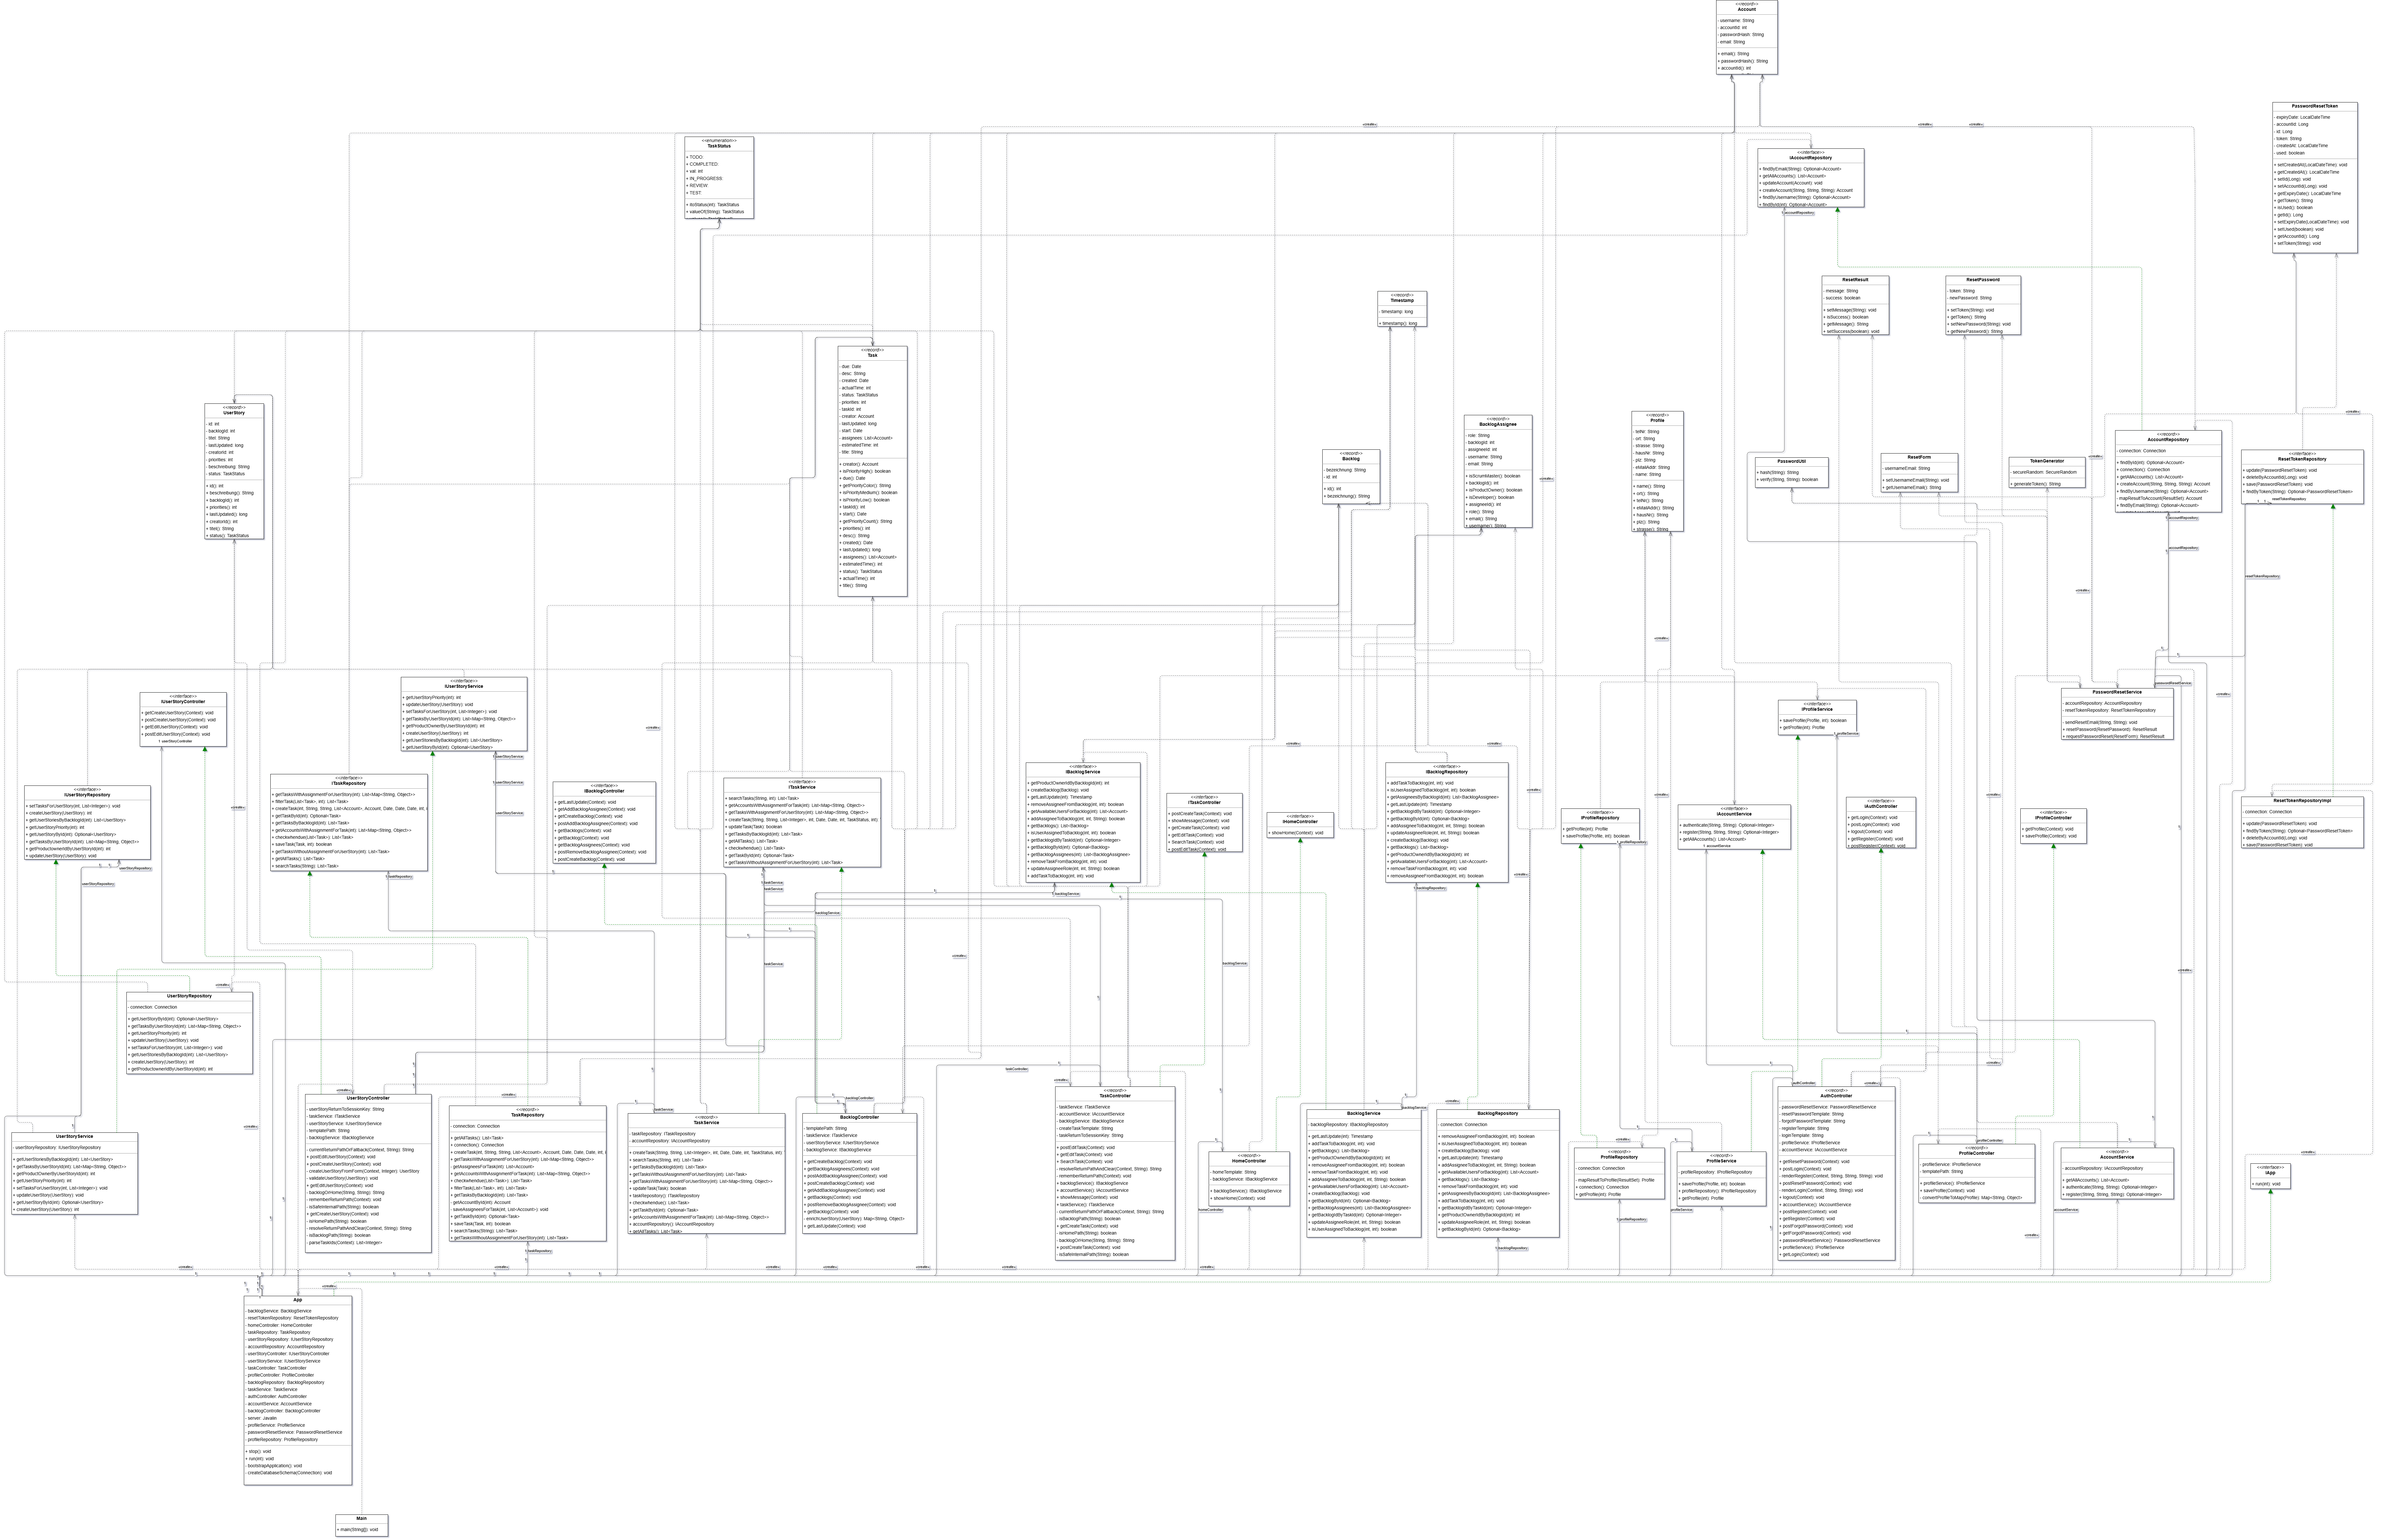
\includegraphics[scale=0.017]{images/layered.drawio.png}};
					\node[draw, rect] (app) at (0,  0) {Data};
					\node[draw, rect] (prs) at (0, -1) {Service};
					\node[draw, rect] (srv) at (0, -2) {Presentation};
					\node[draw, rect] (dat) at (0, -3) {Application};
					
					\node (S) at (3, -1.5) {};
					\spy on (1.25, -2.15) in node at (S.center);
				\end{tikzpicture}
				%			\caption{In der Planphase vorgesehene Hauptkomponenten}
				\label{fig:plan}
			\end{figure}
			}
		\end{minipage}
		\begin{minipage}{0.49\textwidth}
			\begin{itemize}
				\item Application-Layer: \\
				Konfiguration des Servers (\texttt{App.java})
				\item Presentation-Layer: \\
				Controller-Klassen (\texttt{TaskController.java})
				\item Service-Layer: \\
				Business-Logik in Service-Klassen (\texttt{TaskService.java})
				\item Data-Layer: \\
				Repositories, DB-Schema und Datentypen (\texttt{TaskRepository.java},\texttt{Task.java})
			\end{itemize}
		\end{minipage}
		\centering
	\end{frame}
	\begin{frame}{Kernkomponenten}
		\only<1>{
		\begin{minipage}{0.49\textwidth}
			\begin{figure}[!ht]
				\centering
				\resizebox{1\textwidth}{!}{%
					\begin{tikzpicture}
						\tikzstyle{every node}=[font=\fontsize{14.2pt}{18.5pt}\selectfont]
						\draw [ fill={rgb,255:red,255; green,255; blue,255}, fill opacity=1, dashed] (-25,21.5) rectangle (1,3);
						\node[anchor=north west, align=left, inner xsep=1.000cm, inner ysep=1.060cm, rounded corners=0.020cm] at (-24.85,21.35) {\fontsize{18.2pt}{23.7pt}\selectfont Server};
						\draw [ line width=1pt , rounded corners = 46.2] (-17,19) rectangle (-11,15);
						\node[anchor=center, align=center, inner xsep=0.080cm, inner ysep=0.085cm, rounded corners=0.020cm] at (-14,17) {\fontsize{18.2pt}{23.7pt}\selectfont App};
						\draw [line width=1pt, -{Stealth[scale=2]}, ] (-21,13.5) arc[start angle=-179.39, end angle=-270.61, radius=3.9579]node[pos=0.36,right, fill={rgb,255:red,255; green,255; blue,255}, fill opacity=1, text opacity=1, inner xsep=0.080cm, inner ysep=0.085cm, rounded corners=0.020cm]{Rendering};
						\draw [ line width=1pt , rounded corners = 46.2] (-23,13.5) rectangle (-17,9.5);
						\node[anchor=center, align=center, inner xsep=0.080cm, inner ysep=0.085cm, rounded corners=0.020cm] at (-20,11.5) {\fontsize{18.2pt}{23.7pt}\selectfont Controller};
						\draw [ line width=1pt , rounded corners = 46.2] (-14,13.5) rectangle (-8,9.5);
						\node[anchor=center, align=center, inner xsep=0.080cm, inner ysep=0.085cm, rounded corners=0.020cm] at (-11,11.5) {\fontsize{18.2pt}{23.7pt}\selectfont Service};
						\draw [ line width=1pt , rounded corners = 46.2] (-14,8) rectangle (-8,4);
						\node[anchor=center, align=center, inner xsep=0.080cm, inner ysep=0.085cm, rounded corners=0.020cm] at (-11,6) {\fontsize{18.2pt}{23.7pt}\selectfont Repository};
						\draw [ line width=1pt , rounded corners = 46.2] (-23,8) rectangle (-17,4);
						\node[anchor=center, align=center, inner xsep=0.080cm, inner ysep=0.085cm, rounded corners=0.020cm] at (-20,6) {\fontsize{18.2pt}{23.7pt}\selectfont Data Structure};
						\draw [ line width=1pt ] (-7,10) -- (-1,10) -- (-0.5,7) -- (-6.5,7) -- cycle;
						\node [font=\fontsize{18.2pt}{23.7pt}\selectfont, inner xsep=0.080cm, inner ysep=0.085cm, rounded corners=0.020cm] at (-3.5,8.5) {Database}; 
						\draw [line width=1pt, {Stealth[scale=2]}-, ] (-14,11.5) -- (-17,11.5)node[pos=0.5,below, fill={rgb,255:red,255; green,255; blue,255}, fill opacity=1, text opacity=1, inner xsep=0.080cm, inner ysep=0.085cm, rounded corners=0.020cm]{Kontext / Formulardaten};
						\draw [line width=1pt, {Stealth[scale=2]}-, ] (-21.5,13.5) arc[start angle=-179.47, end angle=-270.53, radius=4.4591]node[pos=0.62,left, fill={rgb,255:red,255; green,255; blue,255}, fill opacity=1, text opacity=1, inner xsep=0.080cm, inner ysep=0.085cm, rounded corners=0.020cm]{Kontext / Formulardaten};
						\draw [line width=1pt, {Stealth[scale=2]}-{Stealth[scale=2]}, ] (-4,7) |- (-8,6);
						\draw [line width=1pt, {Stealth[scale=2]}-, ] (-10.5,9.5) arc[start angle=11.44, end angle=-11.44, radius=3.7818]node[pos=0.5,right, fill={rgb,255:red,255; green,255; blue,255}, fill opacity=1, text opacity=1, inner xsep=0.080cm, inner ysep=0.085cm, rounded corners=0.020cm]{Abrufen};
						\draw [line width=1pt, {Stealth[scale=2]}-, ] (-11.5,8) arc[start angle=-168.63, end angle=-191.37, radius=3.8035]node[pos=0.5,left, fill={rgb,255:red,255; green,255; blue,255}, fill opacity=1, text opacity=1, inner xsep=0.080cm, inner ysep=0.085cm, rounded corners=0.020cm]{Speichern};
						\draw [ line width=1pt ] (-8.5,25.5) -- (-2.5,25.5) -- (-2,22.5) -- (-8,22.5) -- cycle;
						\node [font=\fontsize{18.2pt}{23.7pt}\selectfont, inner xsep=0.080cm, inner ysep=0.085cm, rounded corners=0.020cm] at (-5,24) {Client}; 
						\draw [line width=1pt, {Stealth[scale=2]}-{Stealth[scale=2]}, dashed] (-5,22.5) arc[start angle=-2.97, end angle=-92.01, radius=5.8046]node[pos=0.5, fill={rgb,255:red,255; green,255; blue,255}, fill opacity=1, text opacity=1, inner xsep=0.200cm, inner ysep=0.212cm, rounded corners=0.020cm]{GET /\hspace{0.320cm}POST};
						\draw [line width=1pt, -{Stealth[scale=2]}, ] (-14,12) -- (-17,12)node[pos=0.55,above, fill={rgb,255:red,255; green,255; blue,255}, fill opacity=1, text opacity=1, inner xsep=0.080cm, inner ysep=0.085cm, rounded corners=0.020cm]{DB Daten};
						\draw [line width=1pt] (-17,6) -- (-14,6);
					\end{tikzpicture}
				}%
				\label{fig:my_label}
			\end{figure}
		\end{minipage}
		\begin{minipage}{0.49\textwidth}
			\begin{itemize}
				\item App: \\
				Schnittstelle Client $\leftrightarrow$ Server, Definition der Handler, Bootstrapping
				\item Controller: \\
				GET: Holt Daten über Service ein, Rendert diese im Template\\
				POST: Übergibt die Daten aus dem Anwendungskontext an den Service
				\item Service: \\
				Validierung, Transaktionsverwaltung zwischen Controller und Repository
				\item Repository: \\
				DB-Transaktionen
				\item Data Structure: \\
				Strukturbeschreibung
			\end{itemize}
		\end{minipage}
		}
		\only<2>{
		\begin{figure}
			\centering
			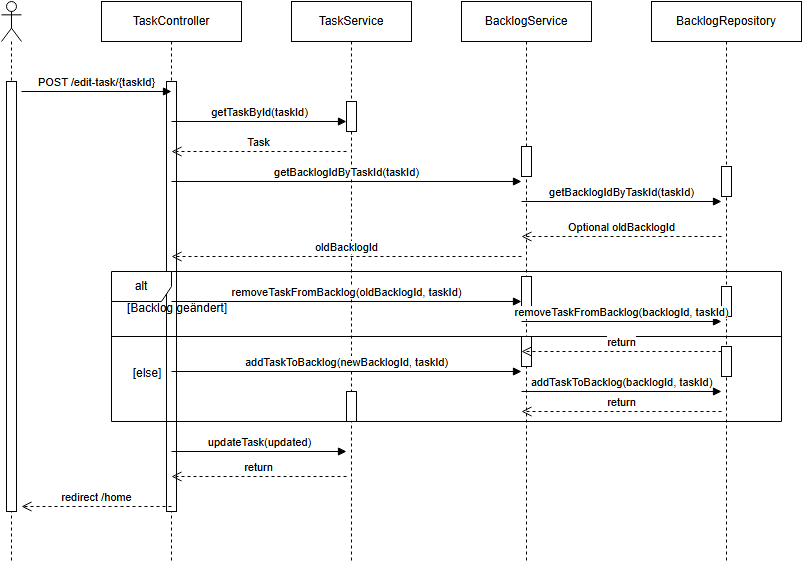
\includegraphics[height=0.8\textheight]{images/s4_3_sequenzdiagramm.png}
%			\caption{Beispielaufruf über alle Schichten}
			\label{fig:d42}
		\end{figure}
		}
	\end{frame}
	
\end{document}
